\chapter{Metodi con intelligenza artificiale}
Negli ultimi anni abbiamo assistito ad uno sviluppo rapidissimo dell’intelligenza artificiale. Nonostante non sia una novità, i recenti avanzamenti tecnologici e la sempre più crescente diponibilità di dati di addestramento, hanno permesso lo sviluppo rapidissimo di queste tecnologie.\\
E anche l’ambito della computer vision e nello specifico della compressione ha seguito questo andamento, infatti negli ultimi anni sono state pubblicate numerose ricerche che vanno a proporre metodi sempre più efficienti per la compressione di immagini tramite l’uso di intelligenze artificiali.\\
Le immagini naturali contengono al loro interno molte ridondanze spaziali che possono essere sfruttate per comprimere senza diminuire la qualità percepita. E le reti neurali sono eccellenti per questo compito. In quanto permettono di ridurre di molto le ridondanze ed identificare le regioni più significative in modo da operare con maggiore precisione su esse.
Partiamo quindi fornendo una rapida introduzione su cosa sia una rete neurale e quali sono i suoi componenti fondamentali.\\
Il componente fondamentale di una rete neurale è l’unita di elaborazione dati chiamata neurone, e più neuroni sono connessi tra di loro tramite connessioni pesate. Solitamente le reti sono composte da più livelli di neuroni e più livelli ci sono più si diche che la rete è profonda. L’analogia con la biologia umana non è casuale, infatti le reti neurali cercano di riprodurre la struttura interna del cervello umano per poterne emulare i processi cognitivi. \cite{sadeeq2021image}\\
Per rendere una rete utilizzabile non è sufficiente crearla definendone la struttura ed altri parametri come le funzioni di attivazione, l’algoritmo di ottimizzazione, il learning rate e altri iperparametri. Ma va addestrata per il compito specifico per la quale la volgiamo utilizzare. Durante la fase di addestramento vengono aggiustati i pesi relativi alle connessioni tra i vari neuroni, questi pesi vengono modificati fino a quando viene trovata la migliore configurazione che raggiunge il miglior risultato possibile nel compito che ci interessa.\\
Durante gli anni si sono sviluppate molte tipologie di reti neurali che si differenziano per configurazione o per metodo di addestramento. In generale però, le reti neurali sono uno dei metodi più comunemente usati per compiti di regressione e classificazione. \cite{sadeeq2021image} Il che le rende sfruttabili per cercare delle funzioni di regressione che permettano di comprimere le informazioni in delle loro rappresentazioni latenti più compresse.
Le strutture che vengono maggiormente utilizzate sono CNN, GAN e Autoencoder. Dei primi due metodi forniremo una breve descrizione per illustrare le differenze principali, mentre sugli Autoencoder ci concentreremo maggiormente in quanto oggetto di questa tesi.
Le reti neurali convoluzionali o CNN sono reti molto indicate per lavorare con immagini o video in quanto estraggono le caratteristiche dai dati di input tramite una serie di livelli convoluzionali e di pooling. Queste caratteristiche vengono poi utilizzate per operazioni di classificazione o identificazione.\\
Le reti avversarie generative o GAN vengono solitamente utilizzate per operazioni di generazione. Queste reti sono costituite da due parti, un generatore e un discriminatore. Il generatore cerca di generare, grazie a ciò che ha appreso dai dati di esempio, nuovi esempi il più realistici possibili per cercare di ingannare il discriminatore. Il discriminatore invece cerca di capire quali esempi sono reali e quali generati. 


\section{Funzionamento degli autoencoder}
Gli autoencoder o autocodficatori sono un modello, le cui prime applicazioni risalgono al 1980, che consiste di due parti un codificatore si occupa di effettuare l’embedding dell’input, ovvero convertire l’input in una sua rappresentazione latente di dimensione inferiore. Da questa rappresentazione il decodificatore cerca di ricostruire l’input nel modo più fedele possibile. Lo schema classico di un autoencoder è visibile nell’immagine \ref{fig:modelloAutoencoder}\\
\begin{figure}[!h]
    \centering
    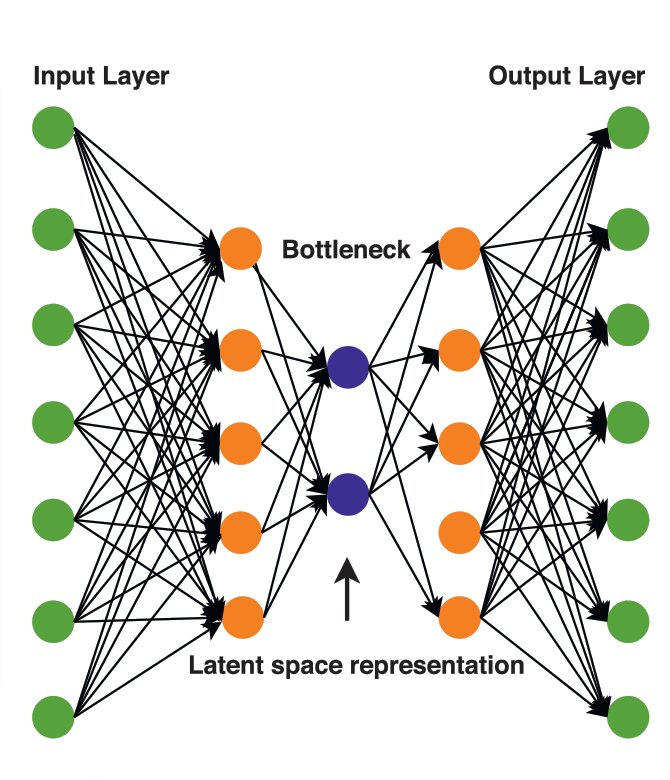
\includegraphics[width=0.5\textwidth]{Immagini/Autoencoder_scheme.png}
    \caption{Diagramma generico di un autoencoder}
    \label{fig:modelloAutoencoder}
\end{figure}\\
Queste reti sono allenate utilizzando delle funzioni di perdita che vanno a misurare la differenza tra i dati in ingresso al codificatore e il prodotto del decodificatore. In base al risultato della funzione di perdita aggiustano i pesi delle reti fino a raggiungere il miglior risultato possibile, ovvero fino a realizzare una ricostruzione il più simile possibile ai dati di input.
Gli autoencoder non sono però sufficienti per costruire un algoritmo di compressione che, come illustrato precedentemente, consiste di almeno elementi e piuù recentemente quattro.
\newpage
\section{Reti di Compressione}
Per ovviare a questo problema sono stati quindi sviluppati i Compressive autoencoder o CAE, che non sono nient’altro che un’estensione degli autoencoder in cui oltre alla rete neurale viene aggiunto un modello di probabilità che si occupa di assegnare un numero di bit alle rappresentazioni in base alla loro frequenza. Questa aggiunta permette di effettuare la codifica entropica della rappresentazione latente. \cite{theis2017lossy}\\
La funzione di perdita di questa nuova architettura \ref{eq:CAELoss} varia leggermente rispetto quella dei soli autoencoder, in quanto viene aggiunto un termine che tiene conto del numero di bit utilizzati. 
\begin{equation}\label{eq:CAELoss}
    L = \underbrace{- \log_{2}(Q([f(x)]))}_{\textrm{numero di bit}} + \beta \cdot \underbrace{d(x,g([f(x)]))}_{\textrm{distorsione}}
\end{equation}\\
Come possiamo vedere, l’equazione consiste di due termini principali, il termine di destra rappresenta la distorsione tra ingresso e uscita della rete. Il secondo termine a sinistra viene introdotto appositamente per le CAE e stima il numero di bit utilizzati, questo permette di ottimizzare la rete non solo in base alla distorsione ma anche in base al numero di bit. Per controllare il compromesso tra numero di bit e distorsione viene introdotto il parametro $\beta$.\\
Il problema con questa nuova funzione nasce dal fatto che durante la fase di backpropagation, con tecniche come Stocastic Gradient Descent (SGD) dove è necessario calcolare il gradiente. La funzione sopra illustrata non può essere utilizzata in quanto composta da funzioni non differenziabili, ovvero la funzione $Q$ e l’arrotondamento $[/dot]$. Per ovviare a questo inconveniente è necessario trovare delle alternative differenziabili.\\
Theis et al. \cite{theis2017lossy} propone due soluzioni possibili, basate sul lavoro di Ballé et al. (2016) \cite{balle2018variational}. La prima soluzione si propone di risolvere il problema della funzione di arrotondamento, mentre Ballé et al. (2016) proponeva invece di utilizzare del rumore additivo gaussiano. \ref{eq:mbtGaussianNoise}.\\
\begin{equation}\label{eq:mbtGaussianNoise}
    [f(x)] \approx f(x) + u
\end{equation}\\
Theis propone invece di rimpiazzare la derivata durante la fase di backpropagation con una sua approssimazione lineare. Empiricamente hanno trovato che la funzione $r(y)=y$ funziona alla pari di molte altre funzioni più elaborate.\\
La seconda soluzione risolve invece il problema della non differenziabilità della funzione di quantizzazione $Q$, utilizzando un’approssimazione continua \ref{eq:theisLinearApprox}.\\
\begin{equation}\label{eq:theisLinearApprox}
    Q(z) = \int_{[-.5,.5[^{M}} q(z+u) du
\end{equation}\\
In questa approssimazione $q$ rappresenta la densità di probabilità della distribuzione $Q$.\\
Lo sviluppo dei compressive autoencoder o CAE e le soluzioni proposte per rendere possibile l’esecuzione di algoritmi di addestramento che richiedono il calcolo dei gradienti delle funzioni di perdita. Hanno permesso di sviluppare, negli anni successivi modelli e nuove soluzioni in grado di ottenere buone prestazioni rispetto agli algoritmi tradizionali. Una lista che comprende tutti i metodi sviluppati fino al 2022 è presente nel lavoro di Mishra et al. \cite{mishra2022deep}, noi ci concentreremo sui tre che hanno fornito il contributo maggiore allo sviluppo di questi metodi.


\subsection{Ballé 2018}
Il primo metodo che andiamo ad analizzare è quello proposto nel 2018 da Ballé et al. \cite{minnen2018joint} che prosegue il lavoro di Ballè del 2016 \cite{balle2018variational}, lavoro che ha ispirato anche la soluzione sopra descritta offerta da Theis un anno prima.\\
Il modello proposto da Ballé et al. nel 2018 utilizza un modello di probabilità misto a scala gaussiana o GSM dove i parametri di scala sono condizionati da un iperparametro. Questo modello permette l’addestramento end-to-end, ciò include anche l’ottimizzazione della rappresentazione quantizzata dell’iper parametro, del modello dell’entropia e dell’autoencoder principale.\\
L’innovazione principale che questo modello porta è l’aggiunta dell’iper parametro compresso all’informazione trasmessa, ciò permette al decodificatore di usare un modello dell’entropia condizionato dall’iper parametro. Questo permette di avere un modello per l’entropia dipendente dall’immagine.\\
L’immagine \ref{fig:balle2018Network} mostra l’architettura ad alto livello del modello di compressione, come si può osservare il modello sia composto da due sottoreti.
\begin{figure}[!h]
    \centering
    \includegraphics[width=0.5\textwidth]{Immagini/Ballé2018_Rete.png}
    \caption{Diagramma rete Ballè 2018 et al., immagine presa dal documento \cite{minnen2018joint}}
    \label{fig:balle2018Network}
\end{figure}\\
La prima sottorete è l’autoencoder principale che ricava una rappresentazione latente delle immagini.\\
La seconda invece ricava un modello di probabilità per effettuare la codifica entropica della rappresentazione latente. Combina il \textit{Context Model} con l’iper rete.\\
I dati provenienti dalle due sottoreti vengono combinati dalla rete per i parametri dell’entropia, generando la media e la scala per il modello gaussiano dell’entropia.\\
La funzione di perdita utilizzata da questo modello \ref{eq:mbtLoss1} è molto simile a quella riportata in precedenza per i CAE, dove il parametro $\beta$ viene sostituito dal moltiplicatore di Lagrange $\lambda$ che regola il compromesso tasso-distorsione. E come di consueto l’obbiettivo di addestramento è quello di minimizzare la funzione di perdita rispetto ai parametri del modello.\\
\begin{equation}\label{eq:mbtLoss1}
    R + \lambda \cdot D = \underbrace{\mathbb{E}_{x \sim p_{x}}[-\log_{2} p_{\hat{y}}(\lfloor f(x) \rceil)]}_{\textrm{numero di bit}} + \lambda \cdot \underbrace{\mathbb{E}_{x \sim p_{x}}[d(x,g(\lfloor f(x) \rceil))]}_{\textrm{distorsione}}
\end{equation}\\
L’entropia di ogni rappresentazione latente $\hat{y_{i}}$ viene modellata come una gaussiana convoluta con una distribuzione uniforme, dunque il modello dell’entropia ha la formulazione \ref{eq:mbtEntropy}.
\begin{equation}\label{eq:mbtEntropy}
    p_{\hat{y}}(\hat{y}|\hat{z}) = \prod_{i}(\mathcal{N}(\mu_{i},\sigma_{i}^{2})*\mathcal{U}(-\tfrac{1}{2},\tfrac{1}{2}))(\hat{y_{i}})
\end{equation}\\
Per predire media e scala della gaussiana invece vengono utilizzati sia l’iper distribuzione, sia il contesto della rappresentazione latente $\hat{y}$.
In questo modello ci aspettiamo che l’iper codificatore e l’iper decodificatore apprendano due funzioni leggermente differenti in quanto lavorano in combinazione con una rete autoregressiva che determina i parametri del modello dell’entropia. Ed essendo sia la rappresentazione latente che la iper-latente parte dell’informazione compressa generata dalla rete l’equazione \ref{eq:mbtLoss1} deve essere leggermente espansa nell' equazione \ref{eq:mbtLoss2}, per includere il costo di codifica degli iper-latenti e utilizzare come distorsione la distanza quadratica media.\\
\begin{equation}\label{eq:mbtLoss2}
    R + \lambda \cdot D = \underbrace{\mathbb{E}_{x \sim p_{x}}[-\log_{2} p_{\hat{y}}(\hat{y})]}_{\textrm{bit(latenti)}} + \underbrace{\mathbb{E}_{x \sim p_{x}}[-\log_{2} p_{\hat{z}}(\hat{z})]}_{\textrm{bit(iper latenti)}} + \lambda \cdot \underbrace{\mathbb{E}_{x \sim p_{x}}||x-\hat{x}||_{2}^{2}}_{\textrm{distorsione}}
\end{equation}\\
Il team di Ballé fornisce anche i dettagli implementativi per i livelli della rete, che abbiamo riportato nella tabella \ref{tab:mbtLayers}.
\begin{table}[!h]
    \centering
    \resizebox{\textwidth}{!}{%
    \begin{tabular}{@{}c|c|c|c|c|c@{}}
    Codificatore & Decodificatoree & \begin{tabular}[c]{@{}c@{}}Iper\\ Codificatore\end{tabular} & \begin{tabular}[c]{@{}c@{}}Iper\\ Decodificatore\end{tabular} & \begin{tabular}[c]{@{}c@{}}Predittore di\\ Contesto\end{tabular} & \begin{tabular}[c]{@{}c@{}}Parametri\\ Entropia\end{tabular} \\ \midrule
    Conv: 5x5 c192 s2 & Deconv: 5x5 c192 s2 & Conv: 3x3 c192 s1 & Deconv: 5x5 c192 s2 & Masked: 5x5 c384 s1 & Conv: 1x1 c640 s1 \\
    GDN & IGDN & Leaky ReLU & Leaky ReLU &  & Leaky ReLU \\
    Conv: 5x5 c192 s2 & Deconv: 5x5 c192 s2 & Conv: 5x5 c192 s2 & Deconv: 5x5 c288 s2 &  & Conv: 1x1 c512 s1 \\
    GDN & IGDN & Leaky ReLU & Leaky ReLU &  & Leaky ReLU \\
    Conv: 5x5 c192 s2 & Deconv: 5x5 c192 s2 & Conv: 5x5 c192 s2 & Deconv: 3x3 c384 s1 &  & Conv: 1x1 c384 s1 \\
    GDN & IGDN &  &  &  &  \\
    Conv: 5x5 c192 s2 & Deconv: 5x5 c3 s2 &  &  &  & 
    \end{tabular}%
    }
    \caption{Ad ogni riga della tabella corrisponde un livello del modello generalizzato, i dati della tabella sono stati ricavati dal documento  \cite{minnen2018joint}}
    \label{tab:mbtLayers}
\end{table}\\
Possiamo vedere degli esempi di compressione con questa rete nelle immagini \ref{fig:mbt2018Example} e \ref{fig:mbt2018_meanExample}, le due immagini sono state prodotte da due versioni diverse della rete, rispettivamente con media della gaussiana variabile e con media della gaussiana fissata a zero.\\
    

\subsection{Cheng 2020}
Il secondo metodo che approfondiremo è quello proposto da Cheng et al. nel 2020 \cite{cheng2020learned}, questo metodo prende come punto di partenza il lavoro di Ballè et al. \cite{minnen2018joint} e lo migliora apportando delle modifiche al modello di probabilità delle rappresentazioni latenti.\\
Il lavoro di Ballè et al. \cite{minnen2018joint} utilizza una distribuzione Gaussiana con media e scala congiunta con un modello autoregressivo \ref{eq:mbtEntropy}. I test svolti dal team di Cheng hanno evidenziato della ridondanza spaziale residua, ridondanza che se possibile eliminare porterebbe a rappresentazioni leggermente ridotte e quindi più efficienti.\\
La loro proposta è quindi quella di utilizzare una miscela di gaussiane con la formulzione \ref{eq:cheng2020Entropy}
\begin{equation}\label{eq:cheng2020Entropy}
    p_{\hat{y}}(\hat{y}|\hat{z}) = (\sum_{k=1}^{K} w_{i}^{(k)} \mathcal{N}(\mu_{i}^{(k)},\sigma_{i}^{2(k)})*\mathcal{U}(-\tfrac{1}{2},\tfrac{1}{2}))(\hat{y_{i}})
\end{equation}\\
Quindi ogni miscela è caratterizzata da tre parametri, un peso $w_{i}^{(k)}$, la media $\mu_{i}^{(k)}$ e la varianza $\sigma_{i}^{2(k)}$
Con questo metodo sono comunque presenti delle ridondanze, ma l’aggiunta dei pesi $w_{i}$ permette al modello di adattarsi alle diverse regioni delle immagini. Inoltre le varianze prodotte con questo metodo sono più piccole rispetto al metodo di Ballè et al. \cite{minnen2018joint}, il che rende il modello più accurato risultando in una rappresentazione compressa dell’immagine che richiede meno bit.\\
L’architettura della rete proposta da Cheng et al. è rappresentata nell’immagine \ref{fig:cheng2020Network}, come possiamo osservare anche qui sono presenti due sottoreti. Una responsabile di ricavare la rappresentazione latente dell’immagine, l’altra di ricavare gli iperparametri.\\
\begin{figure}[!h]
    \centering
    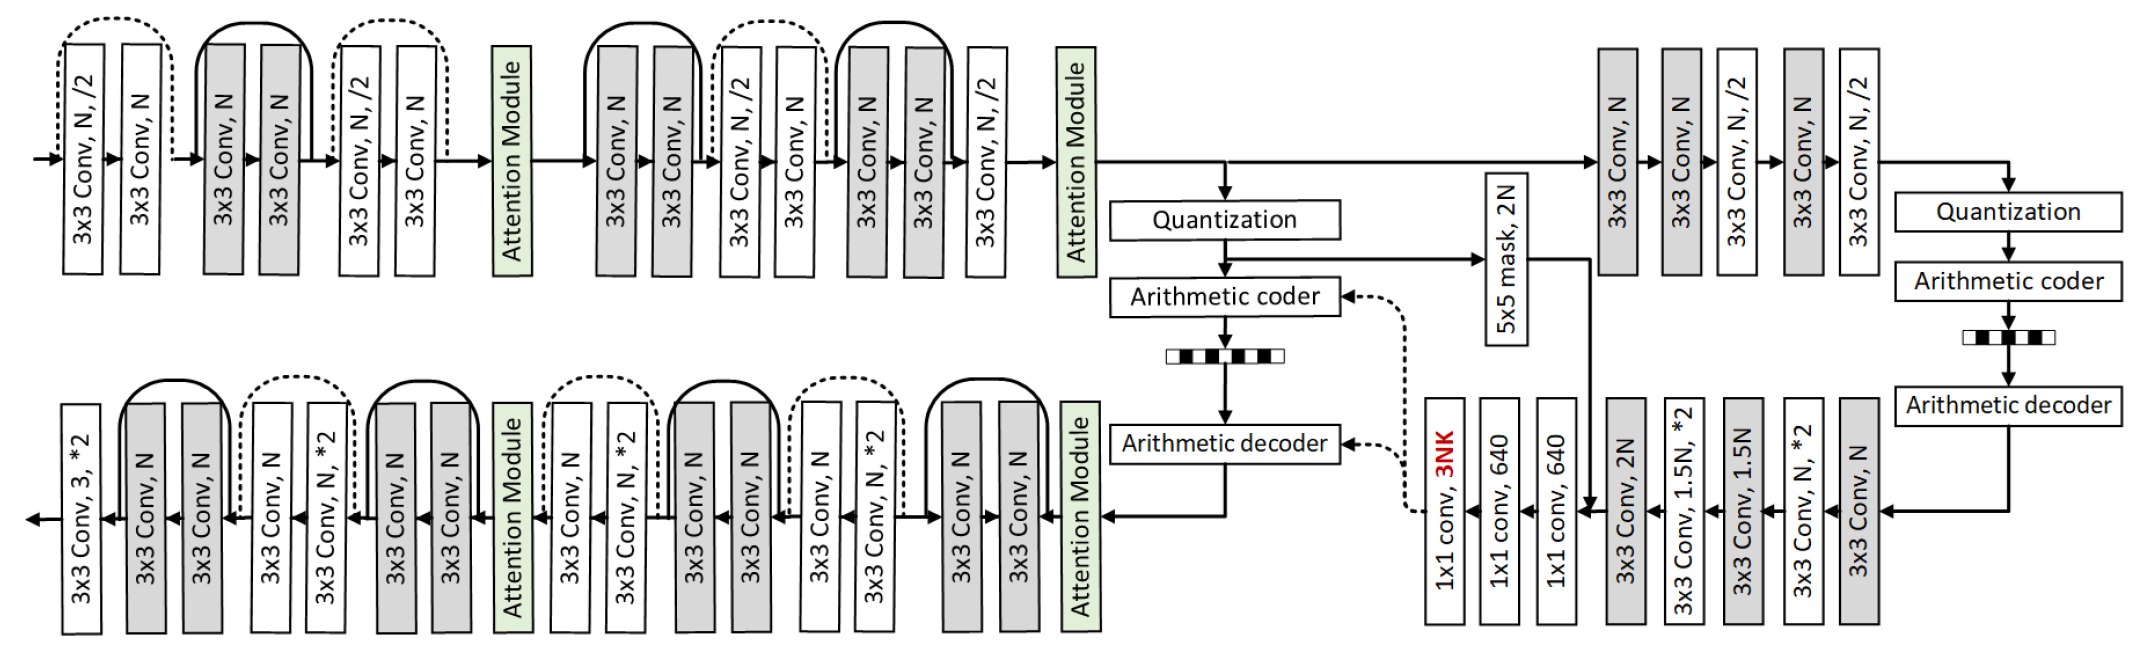
\includegraphics[width=0.9\textwidth]{Immagini/Cheng2020_Rete.png}
    \caption{Diagramma rete Cheng 2020 et al., immagine presa dal documento \cite{cheng2020learned}}
    \label{fig:cheng2020Network}
\end{figure}\\
Questo modello introduce anche due nuovi moduli, gli \textit{Attention Module}, questo moduli servono per aiutare la rete a prestare maggiore attenzione alle parti più complesse delle immagini e ridurre i bit necessari per rappresentare invece le parti più semplici. Uno schema che illustra il funzionamento di un attention module è visibile nell’immagine \ref{fig:cheng2020AttnModuleA}.\\
Questi moduli però richiedono una grande quantità di tempo in fase di addestramento, per cercare di ovviare a questo problema viene proposta una versione semplificata \ref{fig:cheng2020AttnModuleB} in cui è stato rimosso il blocco contenente le informazioni non locali.\\
\begin{figure}[h!]
    \centering
    \begin{subfigure}[]{0.6\textwidth}
        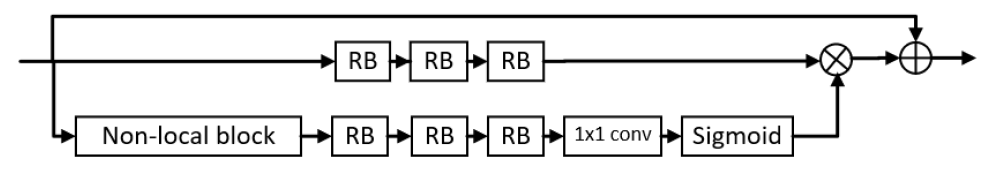
\includegraphics[width=\textwidth]{Immagini/Cheng2020_AttnModuleA.png}
        \caption{Attention module completo}
        \label{fig:cheng2020AttnModuleA}
    \end{subfigure}
    \vspace*{1.5cm}
    \begin{subfigure}[]{0.6\textwidth}
        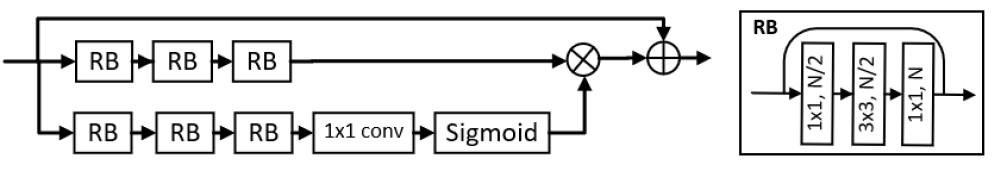
\includegraphics[width=\textwidth]{Immagini/Cheng2020_AttnModuleB.png}
        \caption{Attention module semplificato}
        \label{fig:cheng2020AttnModuleB}
    \end{subfigure}
    \caption{Varianti degli attention modules scviluppati da Cheng 2020 et al., immagine presa dal documento \cite{cheng2020learned}}
    \label{fig:cheng2020AttnModule}
\end{figure}\\
Possiamo vedere degli esempi di compressione con questa rete nelle immagini \ref{fig:cheng2020Example} e \ref{fig:cheng2020_attnExample}, le due immagini sono state prodotte da due versioni diverse della rete, rispettivamente senza \textit{Attnetion module} e con \textit{Attnetion module}.\\
\newpage

\subsection{Wang 2022}
Il terzo ed ultimo metodo che andremo ad approfondire è quello proposto nel 2022 da Wang et al. \cite{wang2022neural}, questo metodo prende i precedenti lavori e cerca di proporre un nuovo approccio per rendere la compressione di un’immagine dipendente dall’immagine stessa. Per fare ciò hanno preso ispirazione di modelli di codifica ibridi e il framework proposto cerca la migliore trasformata per comprimere l’immagine specifica. La proposta di Wang et al. si differenzia dai metodi sviluppati in precedenza nei seguenti aspetti.\\
Durante la fase di codifica vengono prodotti sia la rappresentazione compressa sia una rappresentazione neuro-sintattica, in gradi di catturare informazioni astratte sul contesto dell’immagine che possano aiutare a proiettare la rappresentazione compressa in un sottospazio in cui i coefficienti sono più compatti.\\
Il modello per la codifica entropica si differenzia da quelli esistenti in quanto le due rappresentazioni latenti $\hat{z_{s}}$ e $\hat{z_ {c}}$ vengono codificate separatamente in due stringhe di bit compresse $b_{s}$ e $b_{c}$ con la seguente formula \ref{eq:wang2022LatentEnc}.\\
\begin{equation}\label{eq:wang2022LatentEnc}
    b_{c} = EC (\hat{z_{c}}), \hspace{1 cm} b_{s} =  EC (\hat{z_{s}})
\end{equation}\\
La compressione separata permette un controllo più preciso del processo di codifica. Simmetricamente, il processo di decodifica viene presenta la formulazione \ref{eq:wang2022LatentDec}.\\
\begin{equation}\label{eq:wang2022LatentDec}
    \hat{z_{c}} =  ED (b_{c}), \hspace{1 cm} \hat{z_{s}} =  ED (b_{s}) 
\end{equation}\\
La funzione di decodifica proposta è dipendente dai dati, per immagini di input diverse $x$ si ottengono diverse rappresentazioni neuro-sintattiche $\hat{z_ {s}}$ per generare trasformate di decodifica più specifiche.\\
La funzione di perdita che deve quindi essere ottimizzata in fase di addestramento della rete ha la seguente struttura \ref{eq:wang2022Loss}. Dove $D$ rappresenta la metrica di distorsione e $R$ misura il bit-rate. $\hat{z_{h}}$ rappresenta l’iper distribuzione di $\hat{z_{s}}$ e $\hat{z_{c}}$. $\lambda$ è l’iper parametro che regola il compromesso tra tasso di codifica e distorsione.\\
\begin{equation}\label{eq:wang2022Loss}
    L = D(x,\hat{x}) + \lambda (R(\hat{z_{c}}) +  R(\hat{z_{s}}) + R(\hat{z_{h}}))
\end{equation}\\
La struttura del modello proposto da Wang et al. è visibile nell’immagine \ref{fig:Wang2022Network}, come è possibile osservare ritroviamo la solita struttura composta da due sottoreti, una per di ricavare la rappresentazione latente dell’immagine, l’altra per ricavare gli iperparametri. La novità introdotta in questo modello è la presenza di una trasformata dipendente dai dati in ingresso, questa nuova capacità della rete corrisponde la percorso evidenziato in rosso all’interno della figura \ref{fig:Wang2022Network}.\\
\begin{figure}[!h]
    \centering
    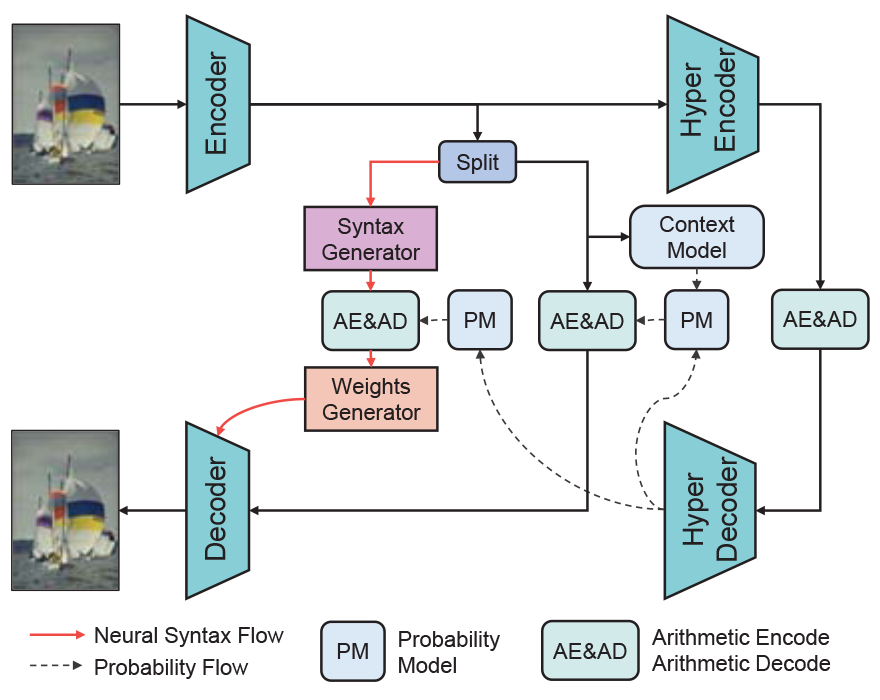
\includegraphics[width=0.6\textwidth]{Immagini/Wang2022_Rete.png}
    \caption{Diagramma rete Wang 2022 et al., immagine presa dal documento \cite{wang2022neural}}
    \label{fig:Wang2022Network}
\end{figure}\\
In questo modello vengono introdotti due nuovi moduli, un \textit{Syntax Generator} e un \textit{Weights Generator} di cui possiamo osservare una rappresentazione nelle immagini \ref{fig:Wang2022SyntaxGenerator} e \ref{fig:Wang2022WeightsGenerator}.\\
\begin{figure}[h!]
    \centering
    \begin{subfigure}[]{0.4\textwidth}
        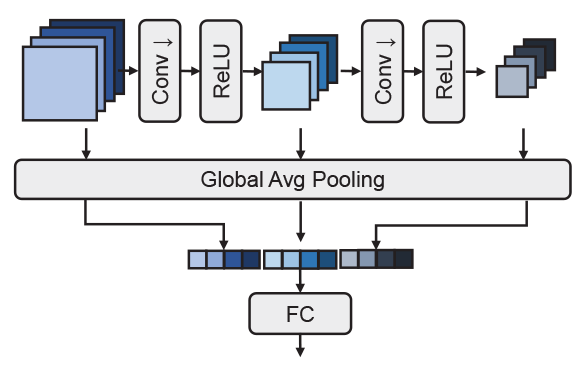
\includegraphics[width=\textwidth]{Immagini/Wang2022_SyntaxGenerator.png}
        \caption{Syntax Generator}
        \label{fig:Wang2022SyntaxGenerator}
    \end{subfigure}
    \hspace*{1 cm}
    \begin{subfigure}[]{0.4\textwidth}
        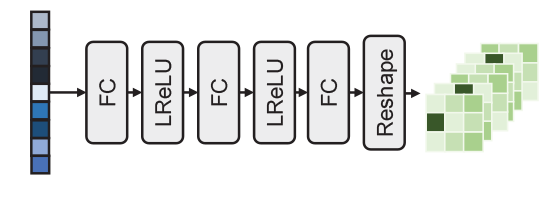
\includegraphics[width=\textwidth]{Immagini/Wang2022_WeightsGenerator.png}
        \caption{Weights Generator}
        \label{fig:Wang2022WeightsGenerator}
    \end{subfigure}
    \caption{Moduli aggiuntivi creati dal tem di Wang et al. per il loro modello, immagini prese dal documento \cite{wang2022neural}}
    \label{fig:Wang2022Modules}
\end{figure}
Il modulo di \textit{Syntax Generation} \ref{fig:Wang2022SyntaxGenerator} è stato creato per estrarre delle informazioni di sintassi dall’input in fase di codifica, dopo averle estratte queste informazioni vengono mappate in un vettore unidimensionale con un operazione di pooling globale. I vettori $\hat{z_{s}}$ vengono quindi concatenati, quantizzati e codificati.\\
Il secondo modulo \ref{fig:Wang2022WeightsGenerator} invece si occupa di mappare la rappresentazione neuro-sintattica $\hat{z_{s}}$ ottenuta durante la codifica in parametri per i kernel della rete di decodifica, l’estrazione di questi parametri è quello che permette a questa rete di creare delle trasformate dipendenti dai dati.\\
Questi parametri vengono utilizzati dalla rete di decodifica, come possiamo vedere nella figura \ref{fig:Wang2022Convolution}, in quanto solo i parametri dell’ultimo livello della rete sono fissati, quelli dei livelli precedenti vengono generati dal \textit{Weights Generator} in modo da permettere alla rete di adattarsi ad immagini diverse.\\
\begin{figure}[!h]
    \centering
    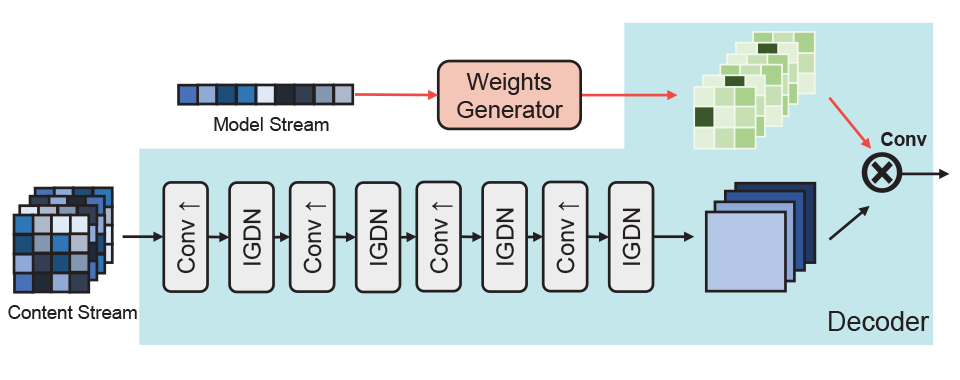
\includegraphics[width=0.5\textwidth]{Immagini/Wang2022_Convolution.png}
    \caption{Convoluzione di pesi e dati nel processo di decodifica nella rete Wang 2022, immagine presa dal documento \cite{wang2022neural}}
    \label{fig:Wang2022Convolution}
\end{figure}\\
Il team di Wang et al. ha inoltre sviluppato un modulo aggiuntivo di post-processing, utile per i casi in cui è richiesta una ricostruzione più dettagliata, anche questa rete fa uso della rappresentazione neuro-sintattica per adattarsi maggiormente alle varie immagini. Grazie a questa aggiunta il team di Wang et al. ha riportato di aver superato anche il codec VVC, che attualmente rappresenta lo stato dell’arte per la compressione di immagini.\\
Di questo modello non possiamo fornire degli esempi di compressione in quanto il team di Wang et al. ha rilasciato il modello ma non la rete pre allenata e non avendo a disposizione dell'equipaggiamento adeguato per eseguire l'allenamento del modello, ci è stao impossibile utilizzare questa rete nei nostri esperimenti.\\
\newpage

\begin{figure}[t!]
    \centering
    \begin{subfigure}[]{0.25\textwidth}
        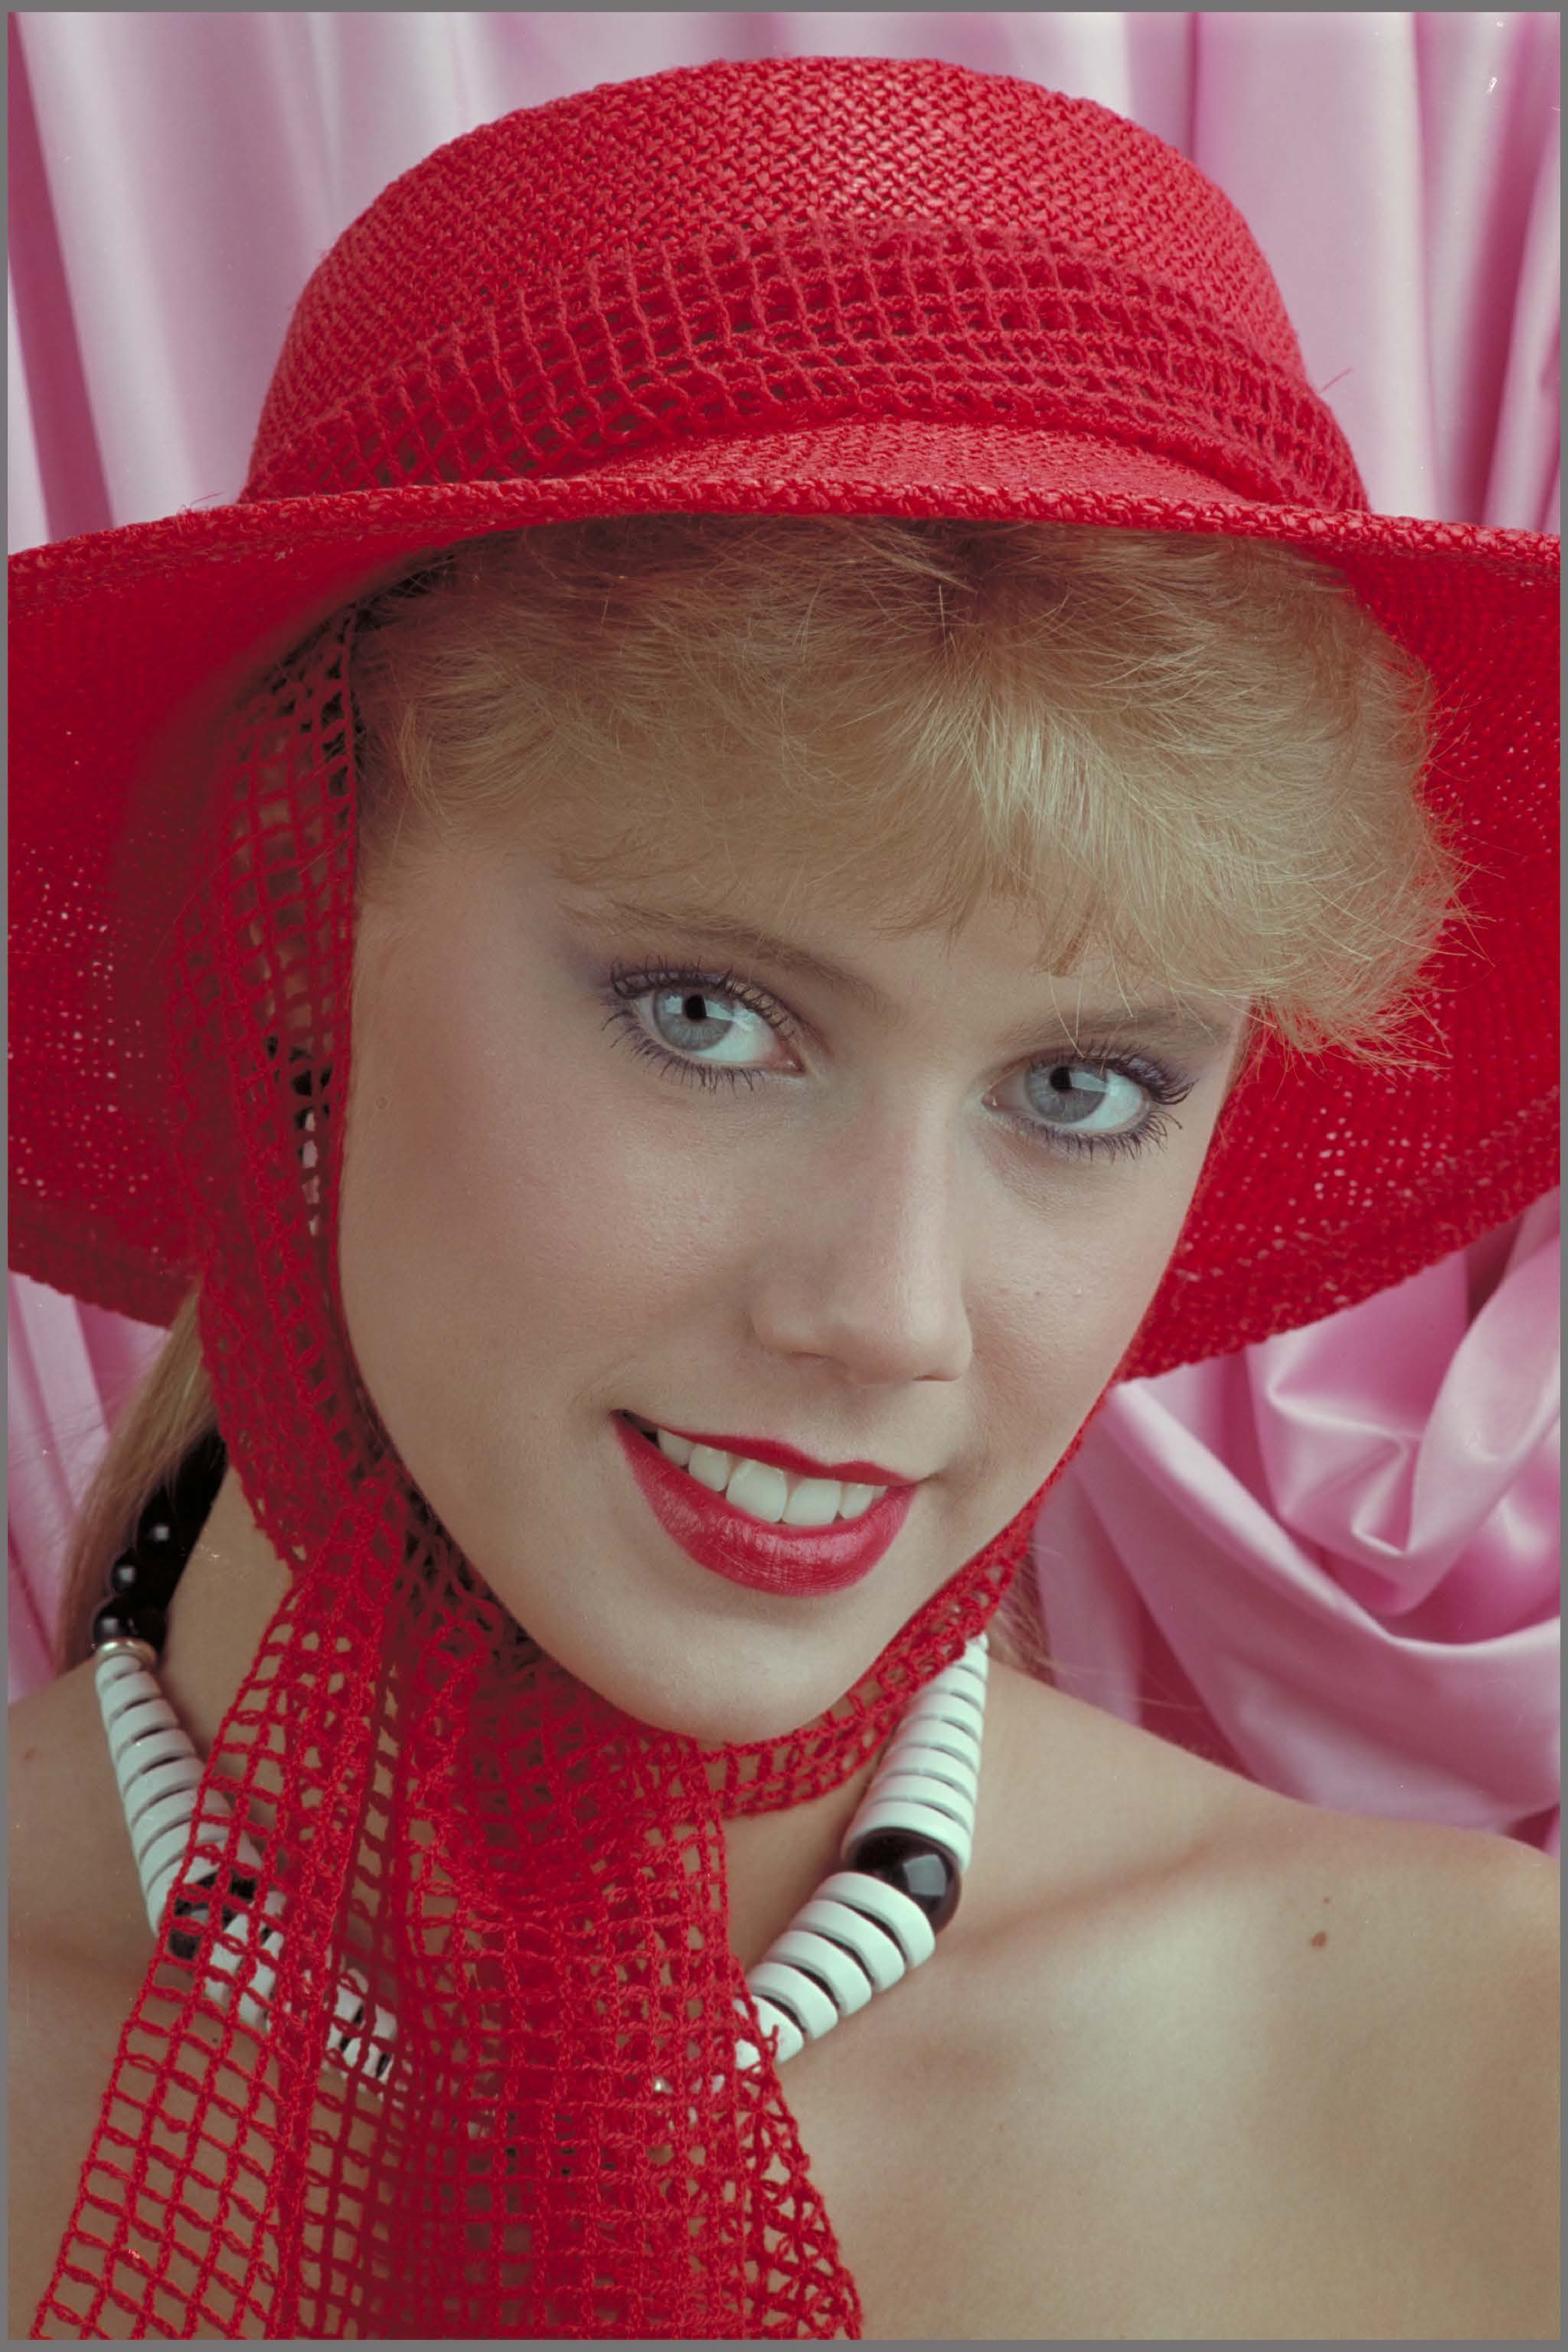
\includegraphics[width=\textwidth]{Immagini/IMAGES/PNG_IMG0004.pdf}
        \caption{Originale}
        \label{fig:OriginalMbt2018}
    \end{subfigure}
    \hspace{0.5cm}
    \begin{subfigure}[]{0.25\textwidth}
        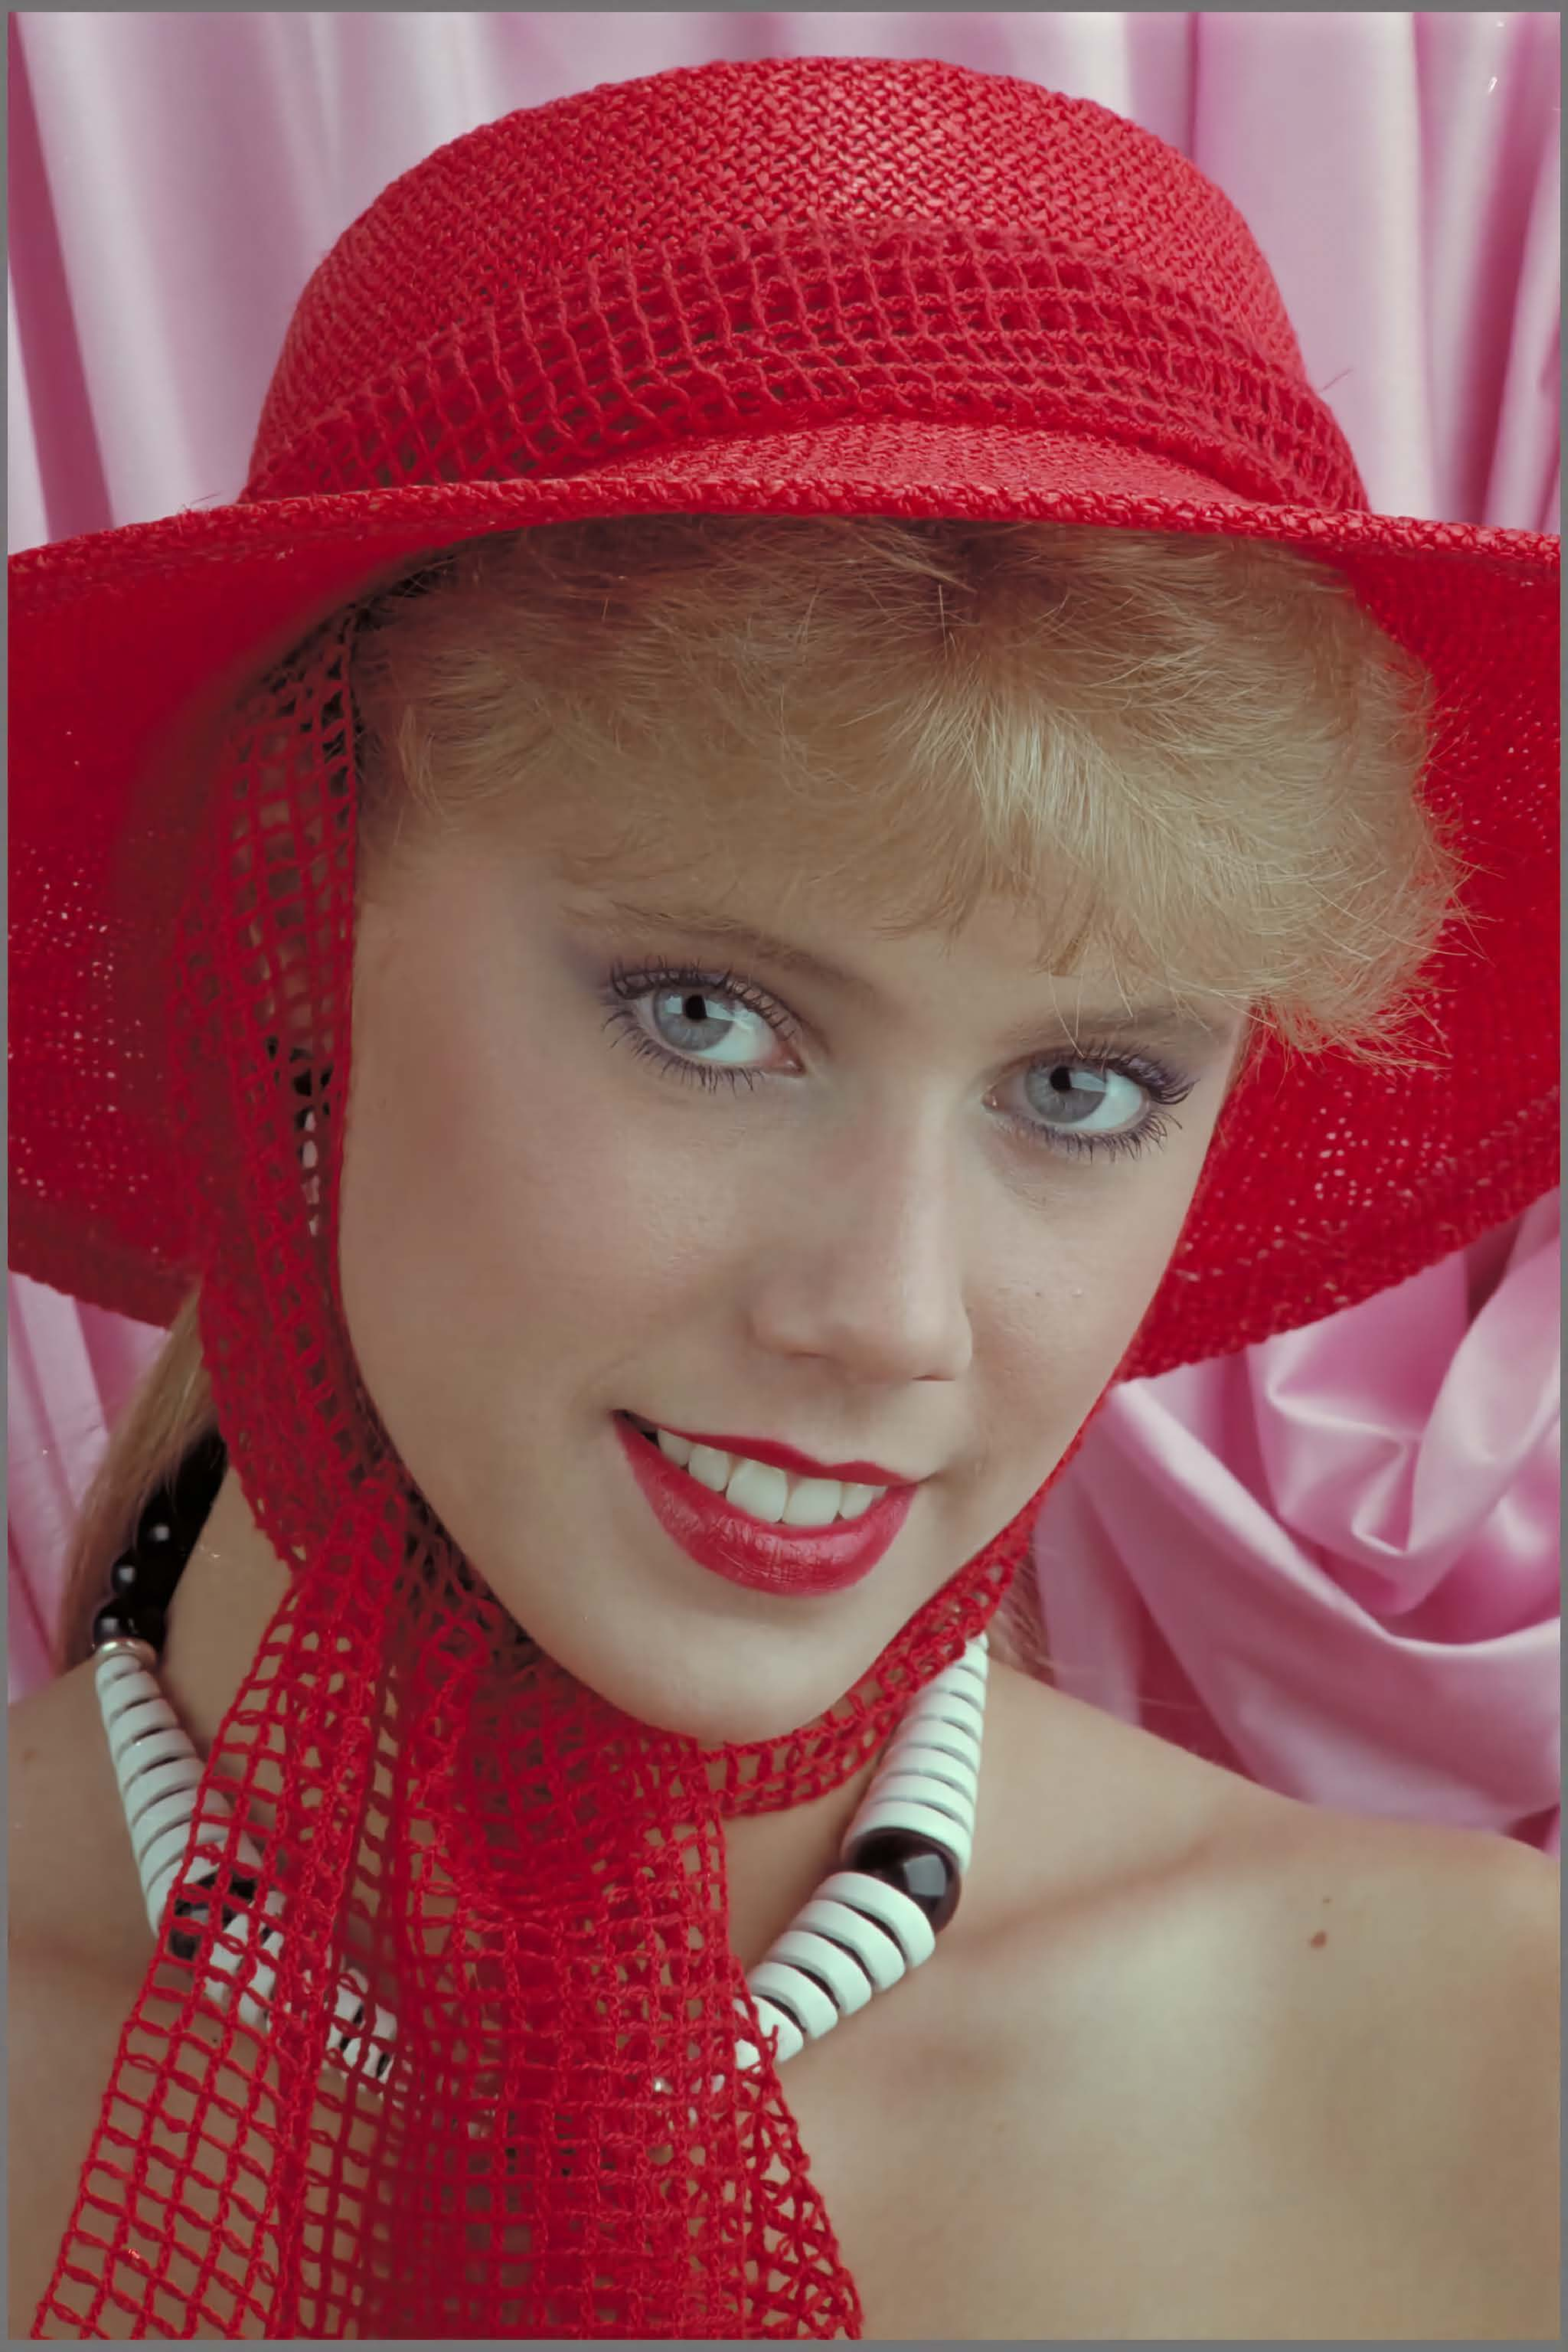
\includegraphics[width=\textwidth]{Immagini/IMAGES/mbt2018_3_IMG0004.pdf}
        \caption{mbt2018}
        \label{fig:CompressedMbt2018}
    \end{subfigure}
    \hspace{0.5cm}
    \begin{subfigure}[]{0.25\textwidth}
        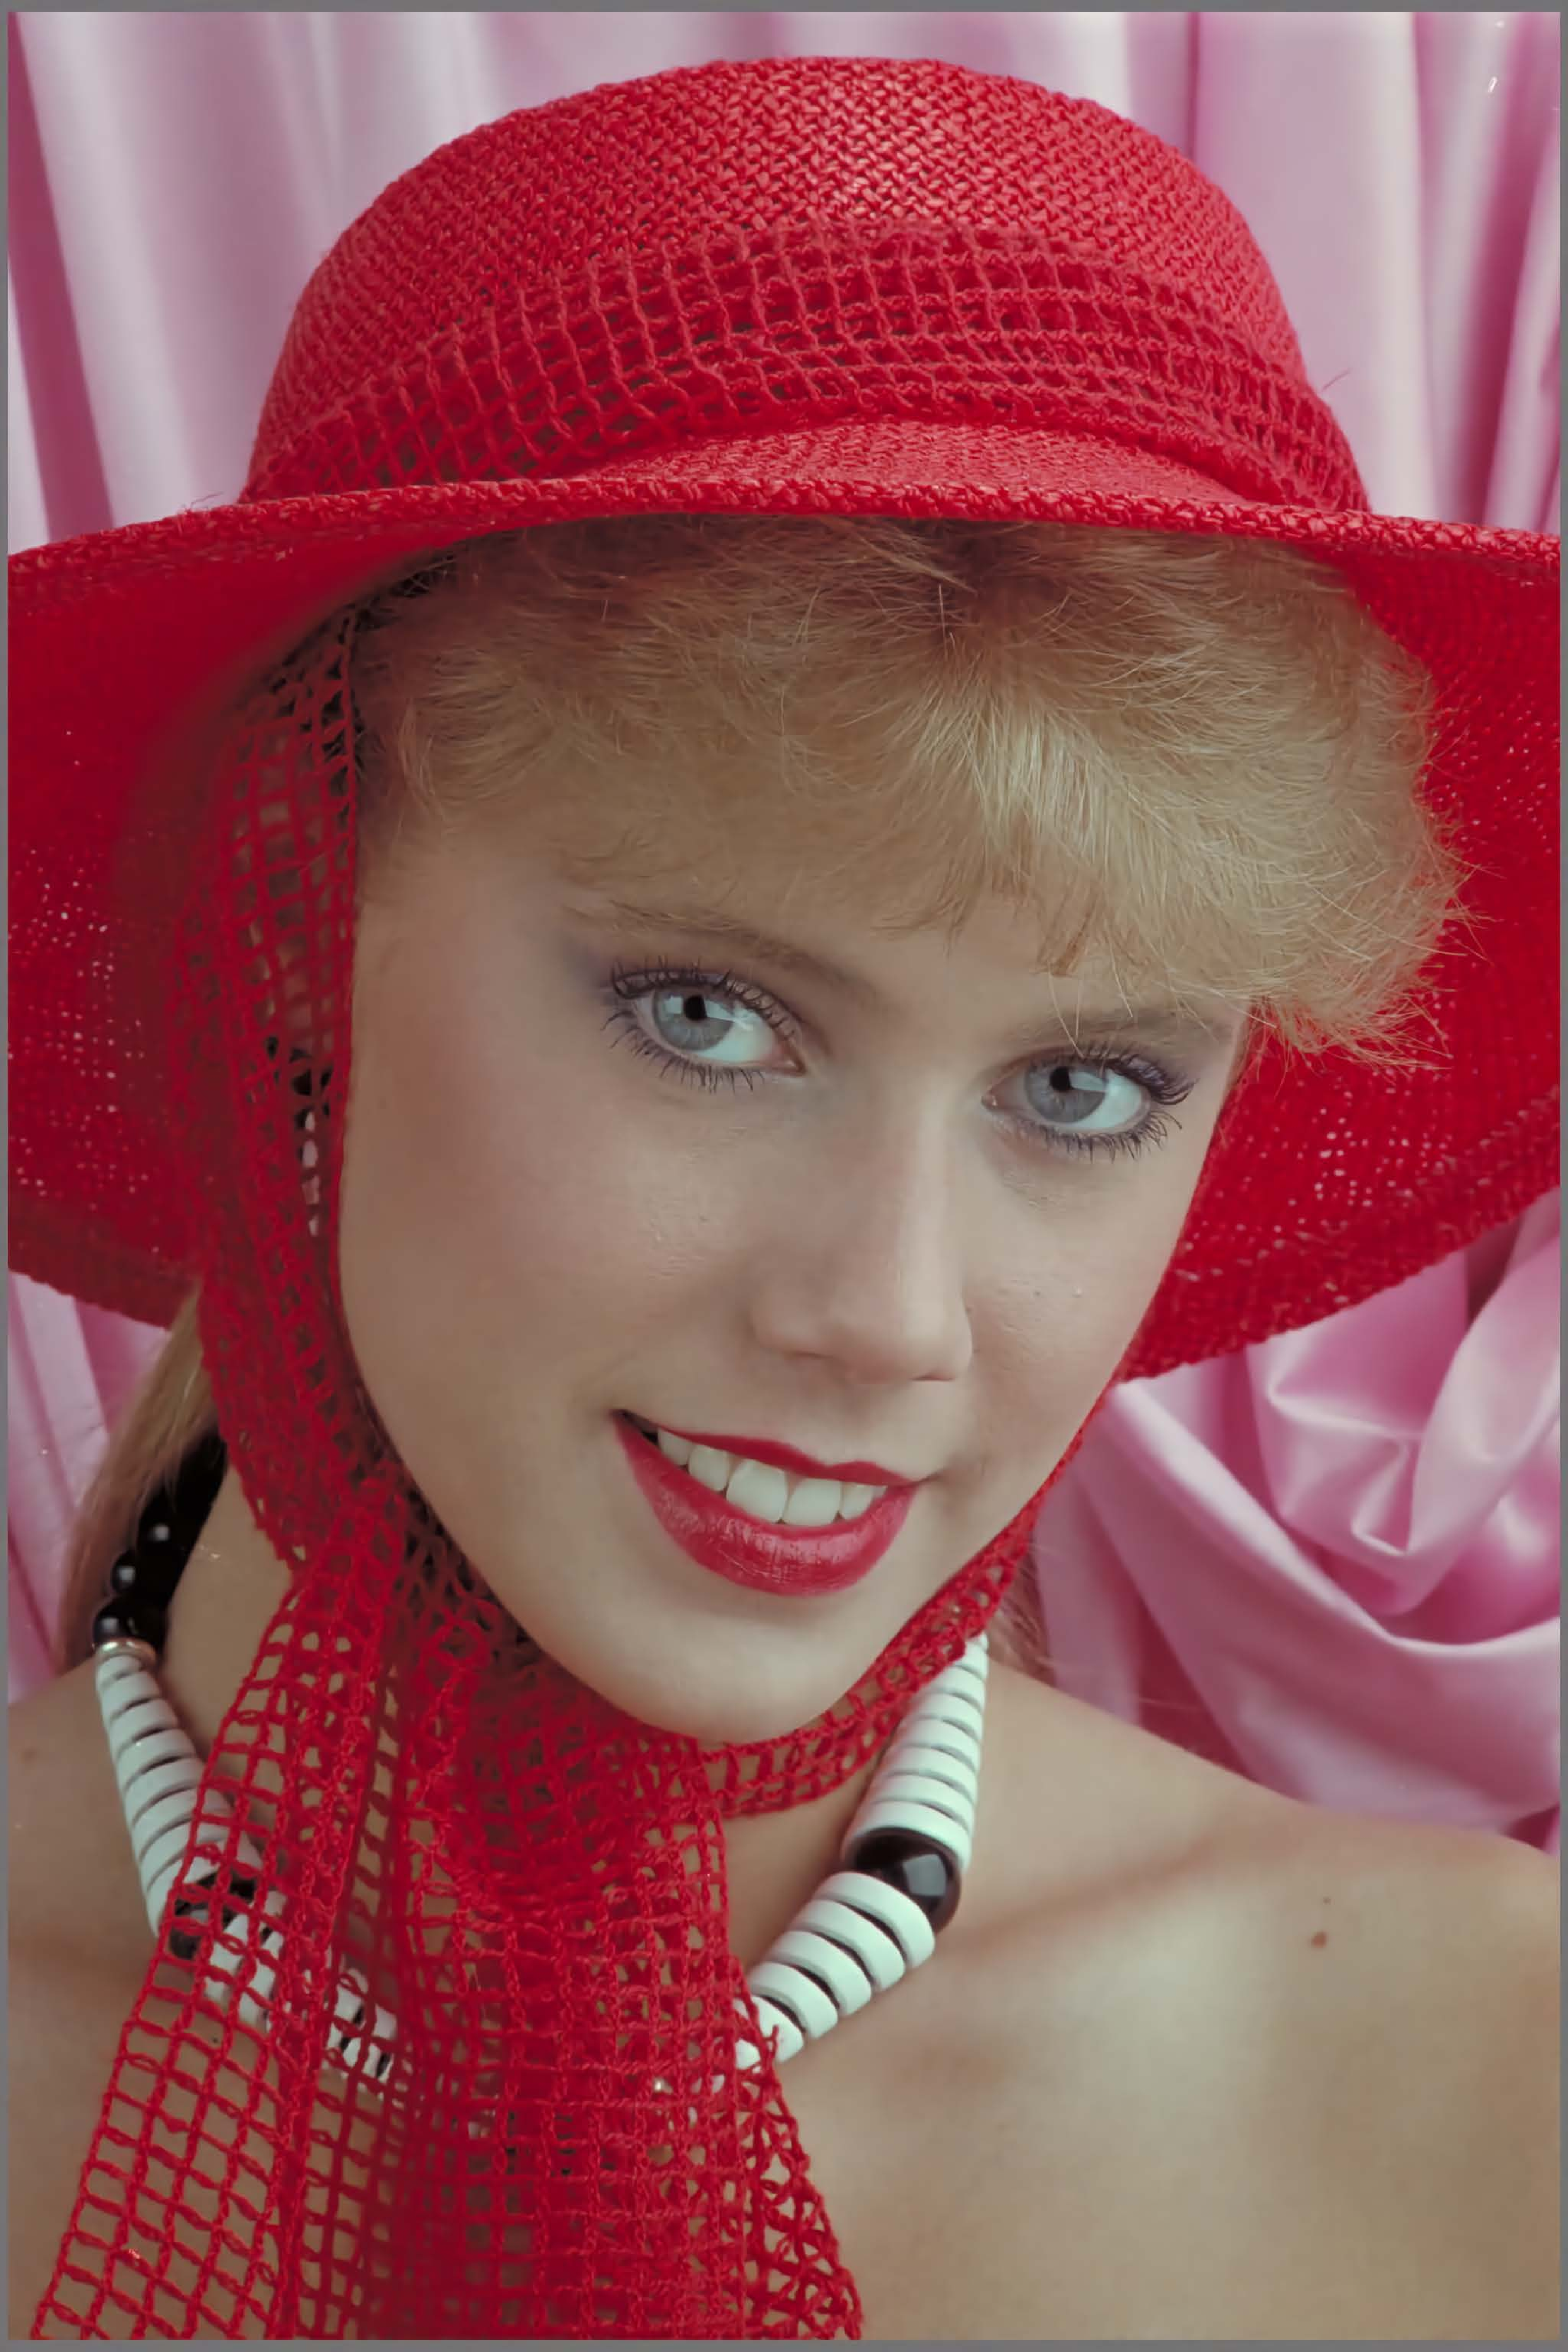
\includegraphics[width=\textwidth]{Immagini/IMAGES/mbt2018_mean_3_IMG0004.pdf}
        \caption{mbt2018 Mean}
        \label{fig:CompressedMbt2018Mean}
    \end{subfigure}
    \caption{Confronto PNG con Ballè 2018 a 0.145 bpp}
    \label{fig:CompressionMbt2018}
\end{figure}

\begin{figure}[t!]
    \centering
    \begin{subfigure}[]{0.25\textwidth}
        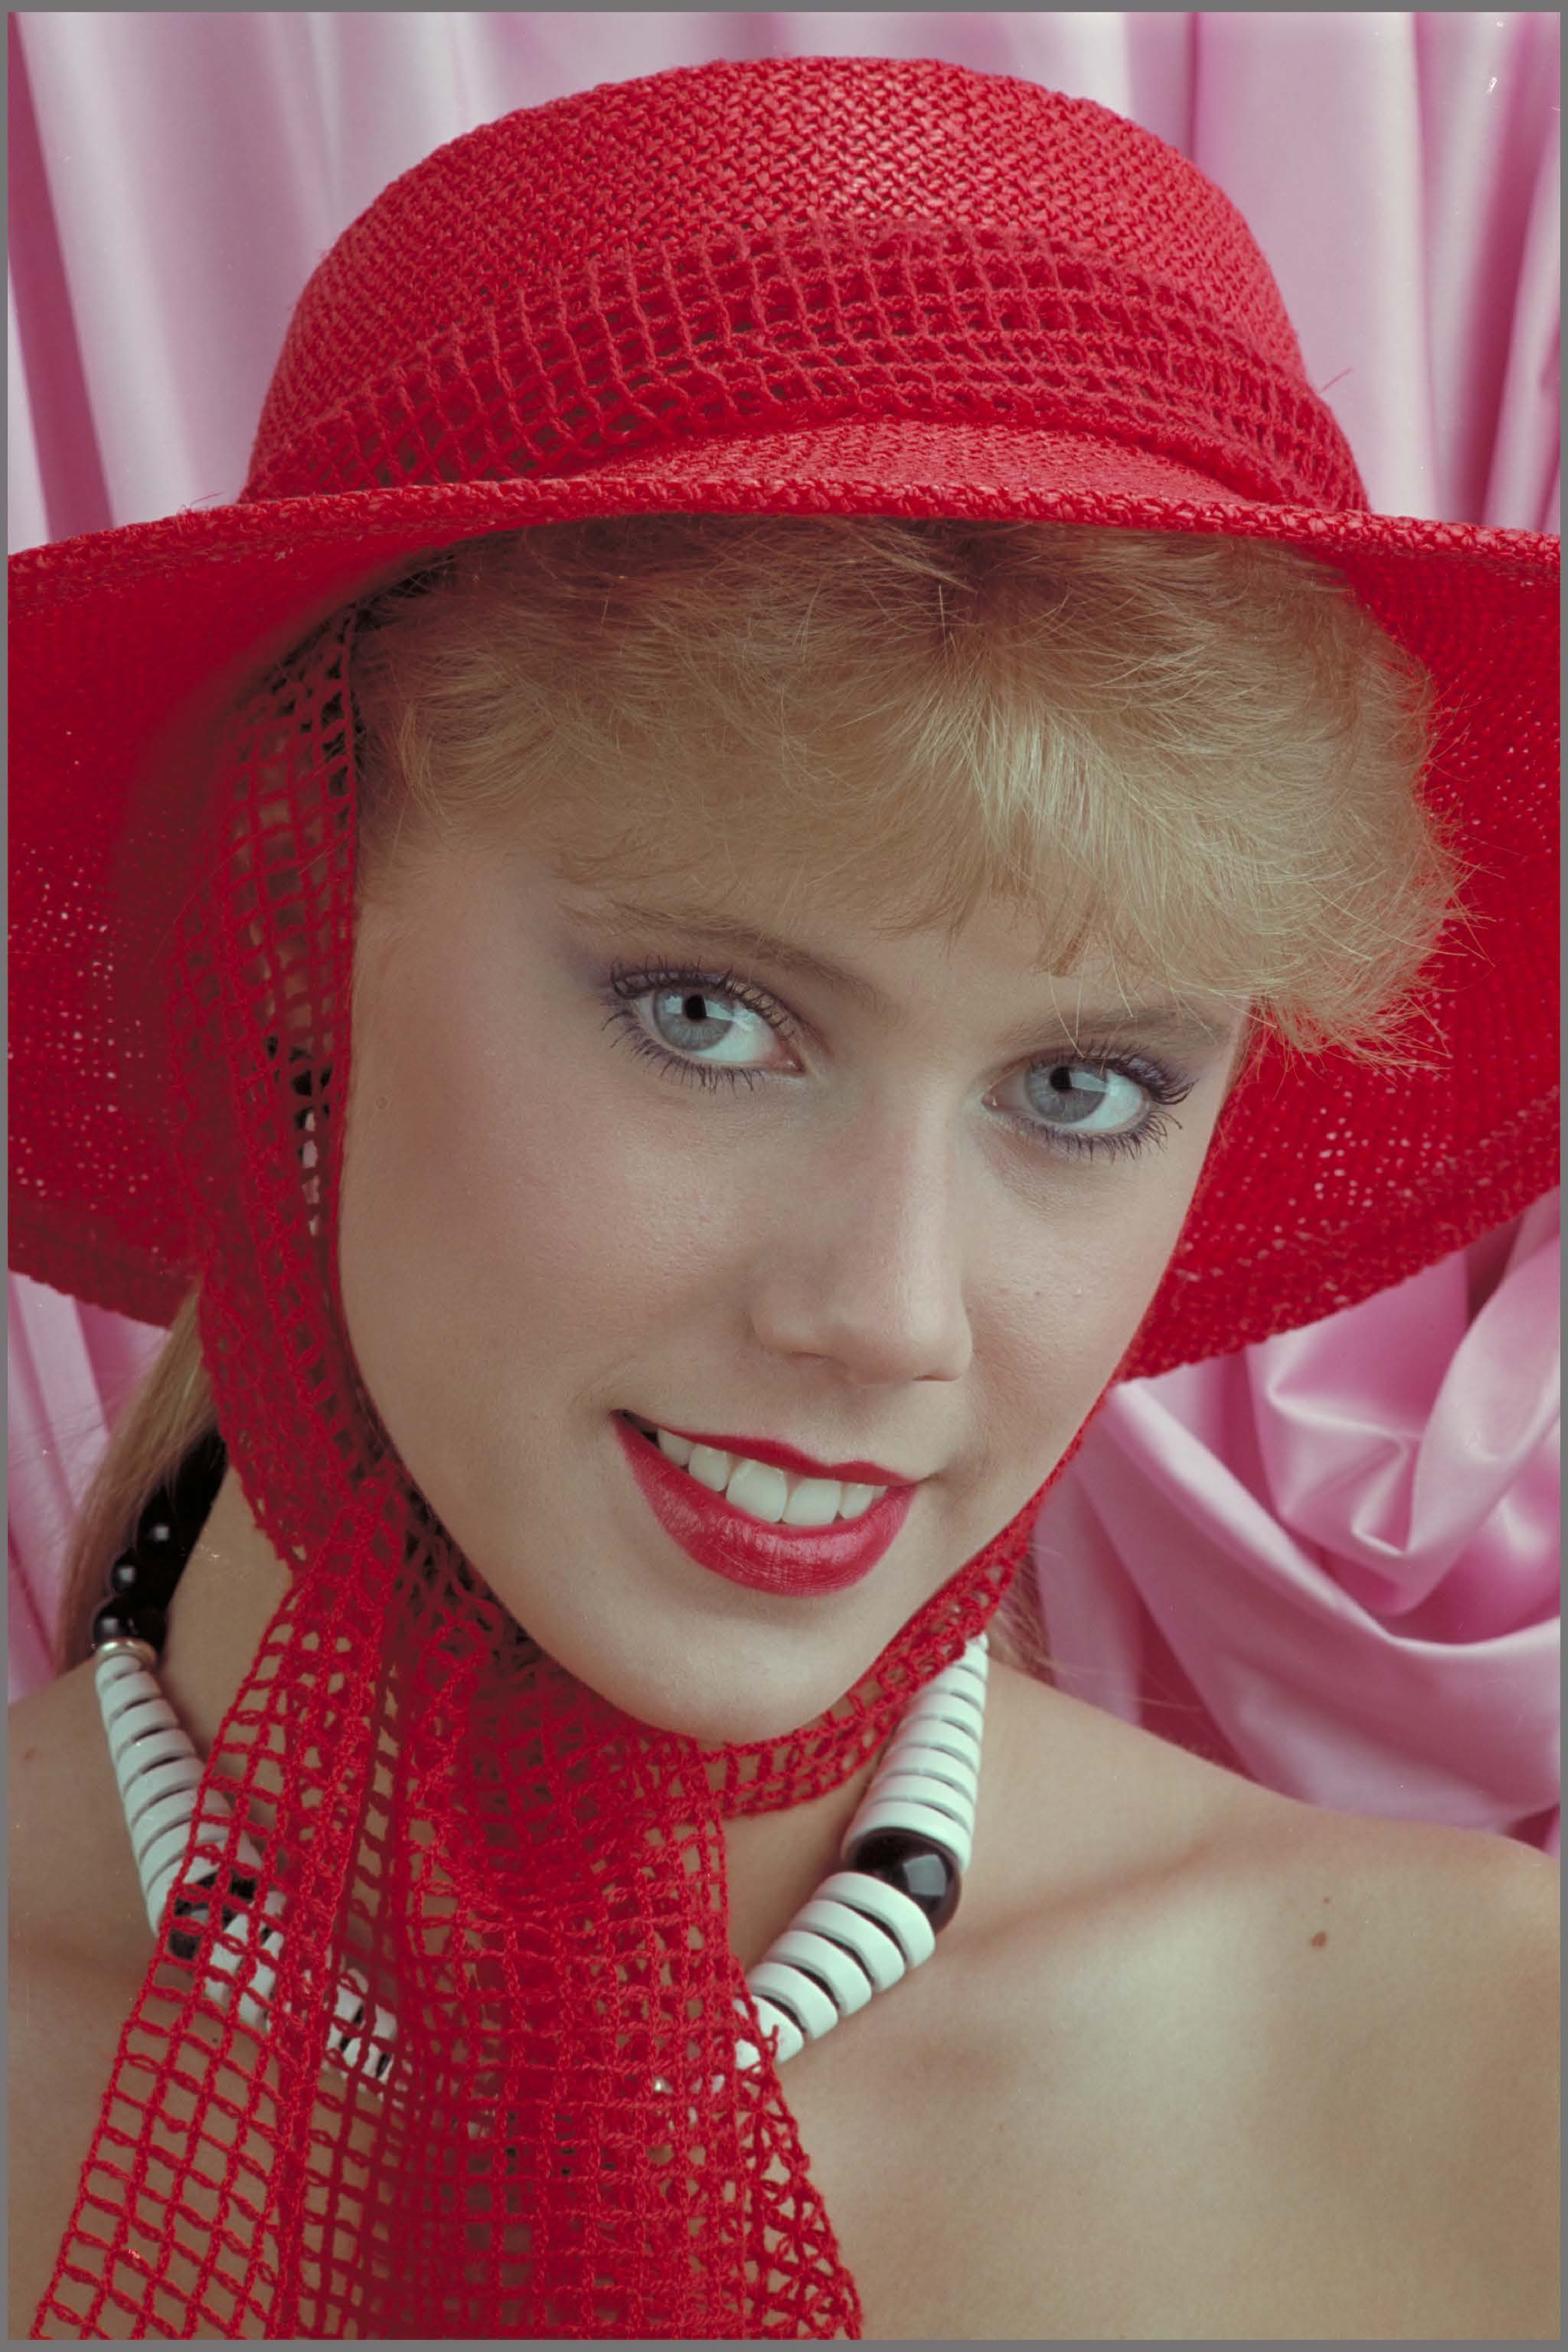
\includegraphics[width=\textwidth]{Immagini/IMAGES/PNG_IMG0004.pdf}
        \caption{Originale}
        \label{fig:OriginalChang2020}
    \end{subfigure}
    \hspace*{0.5cm}
    \begin{subfigure}[]{0.25\textwidth}
        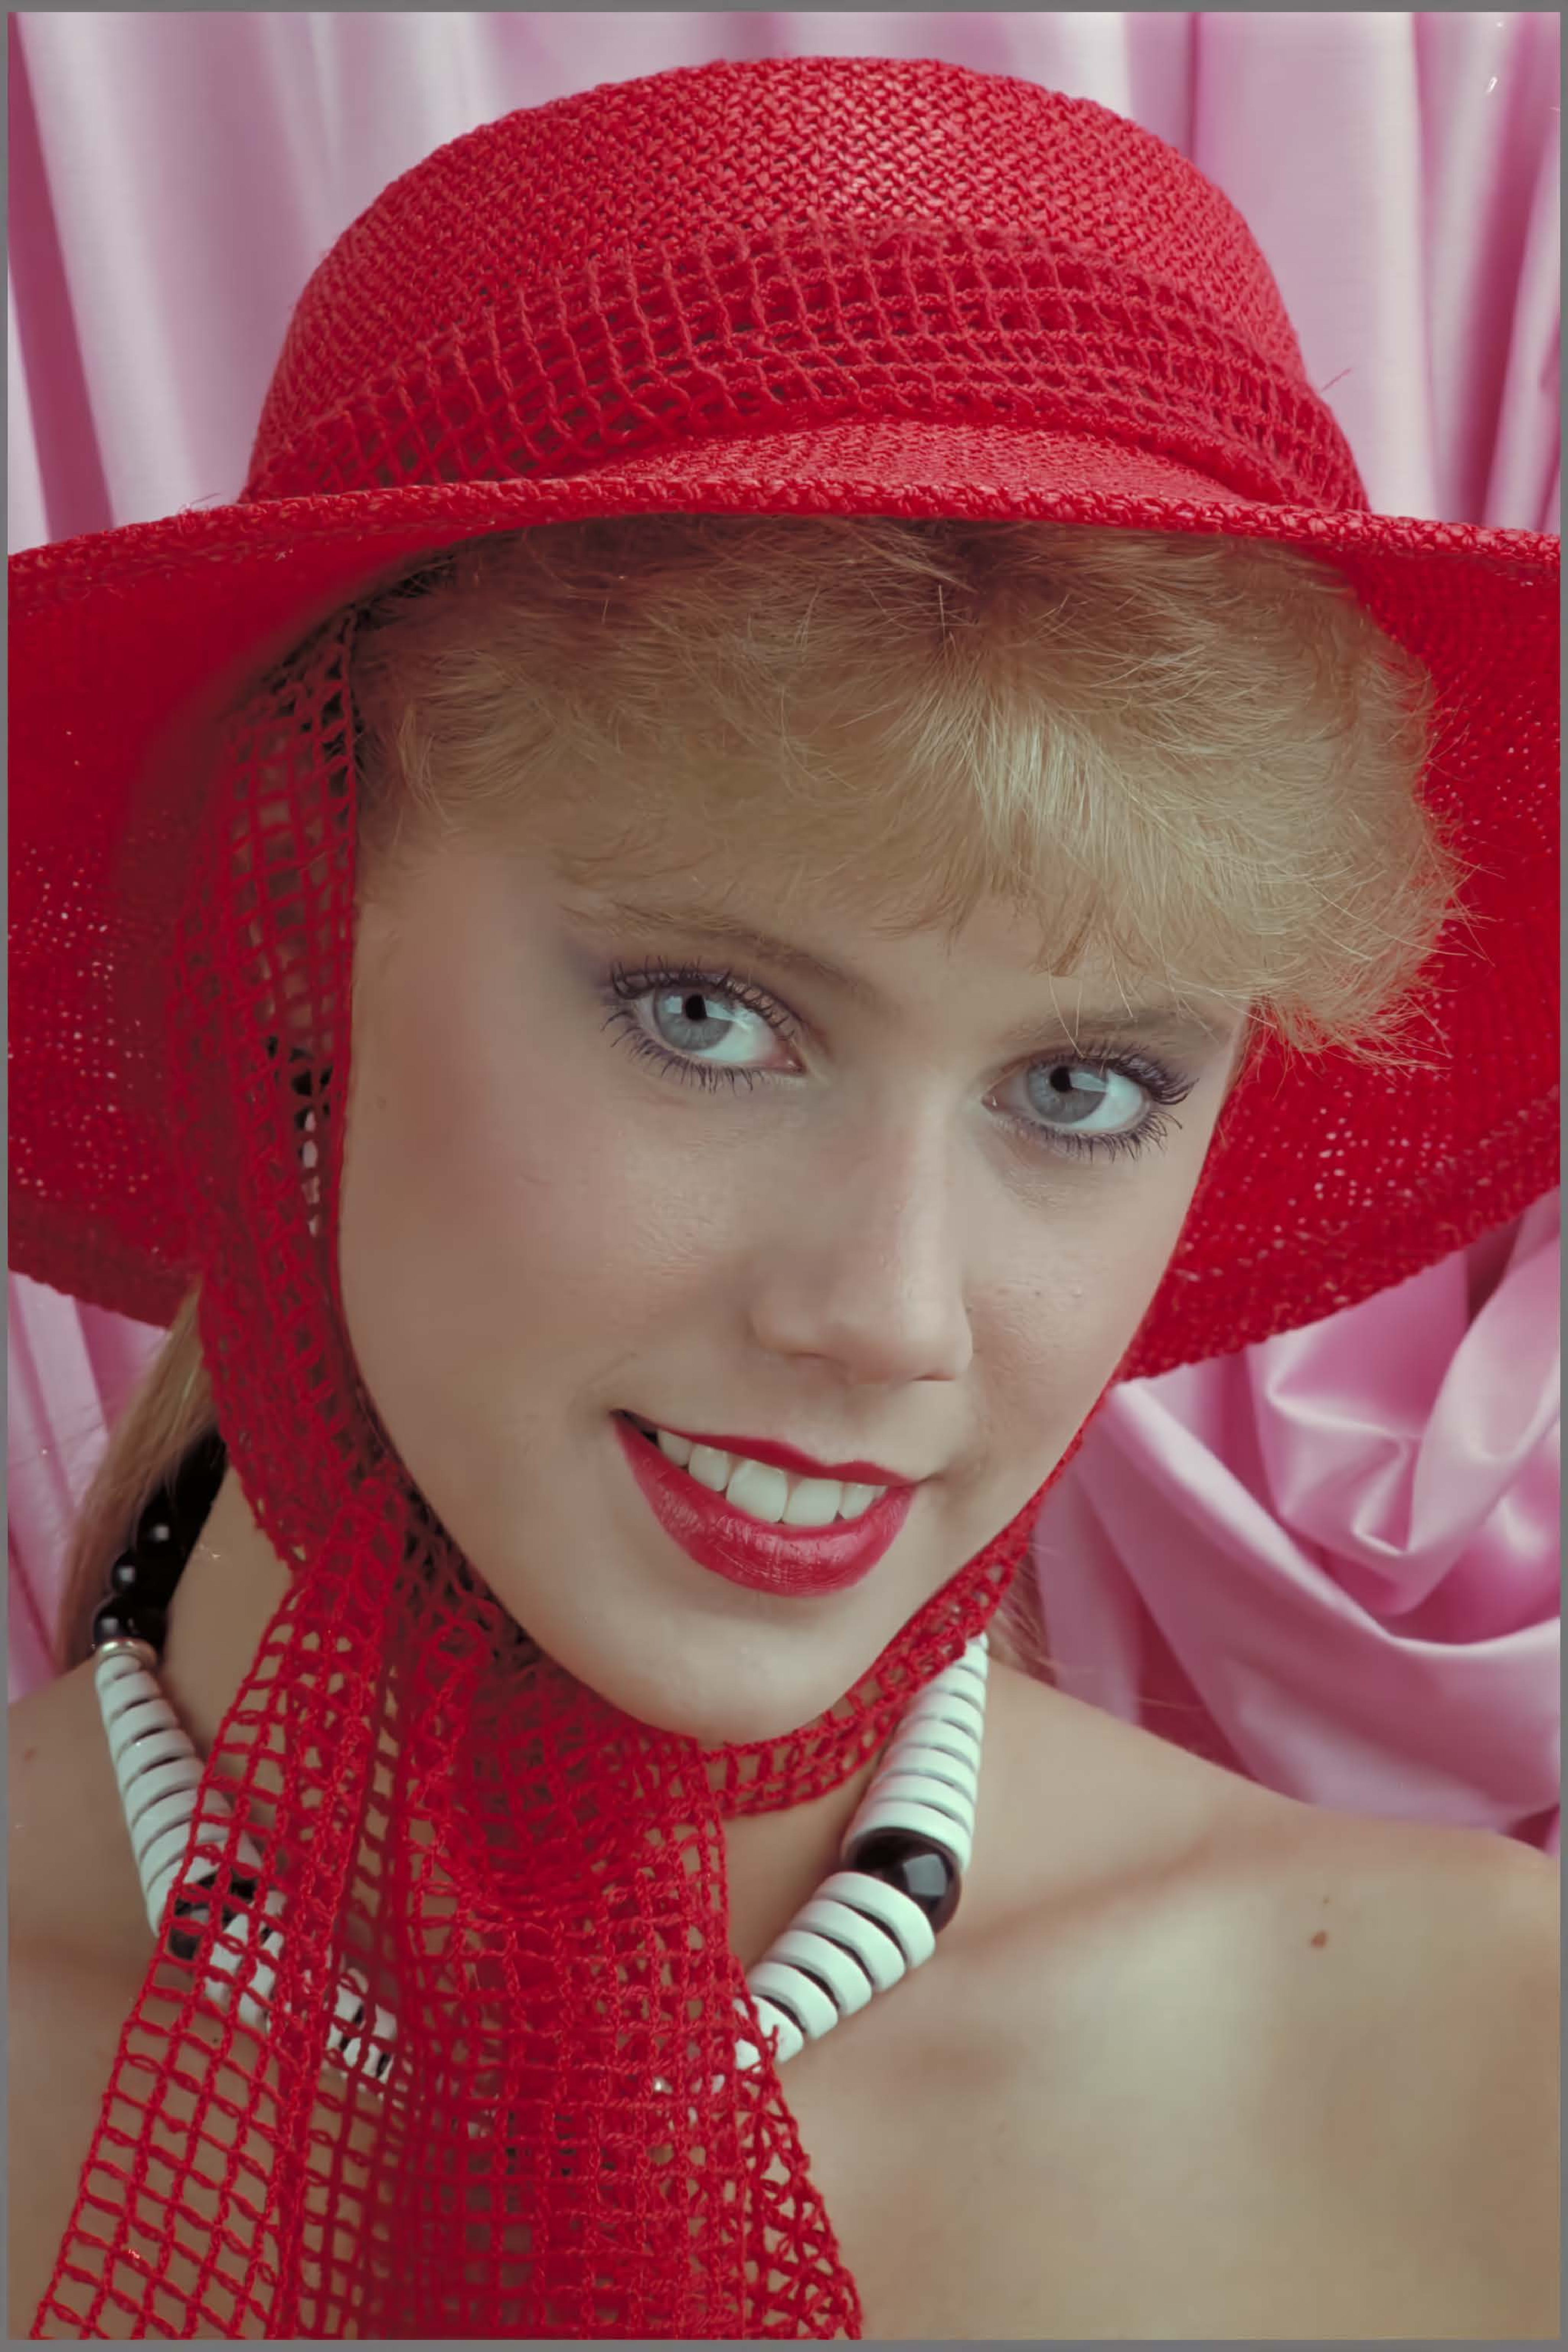
\includegraphics[width=\textwidth]{Immagini/IMAGES/cheng2020_attn_3_IMG0004.pdf}
        \caption{Cheng2020}
        \label{fig:CompressedCheng2020}
    \end{subfigure}
    \hspace*{0.5cm}
    \begin{subfigure}[]{0.25\textwidth}
        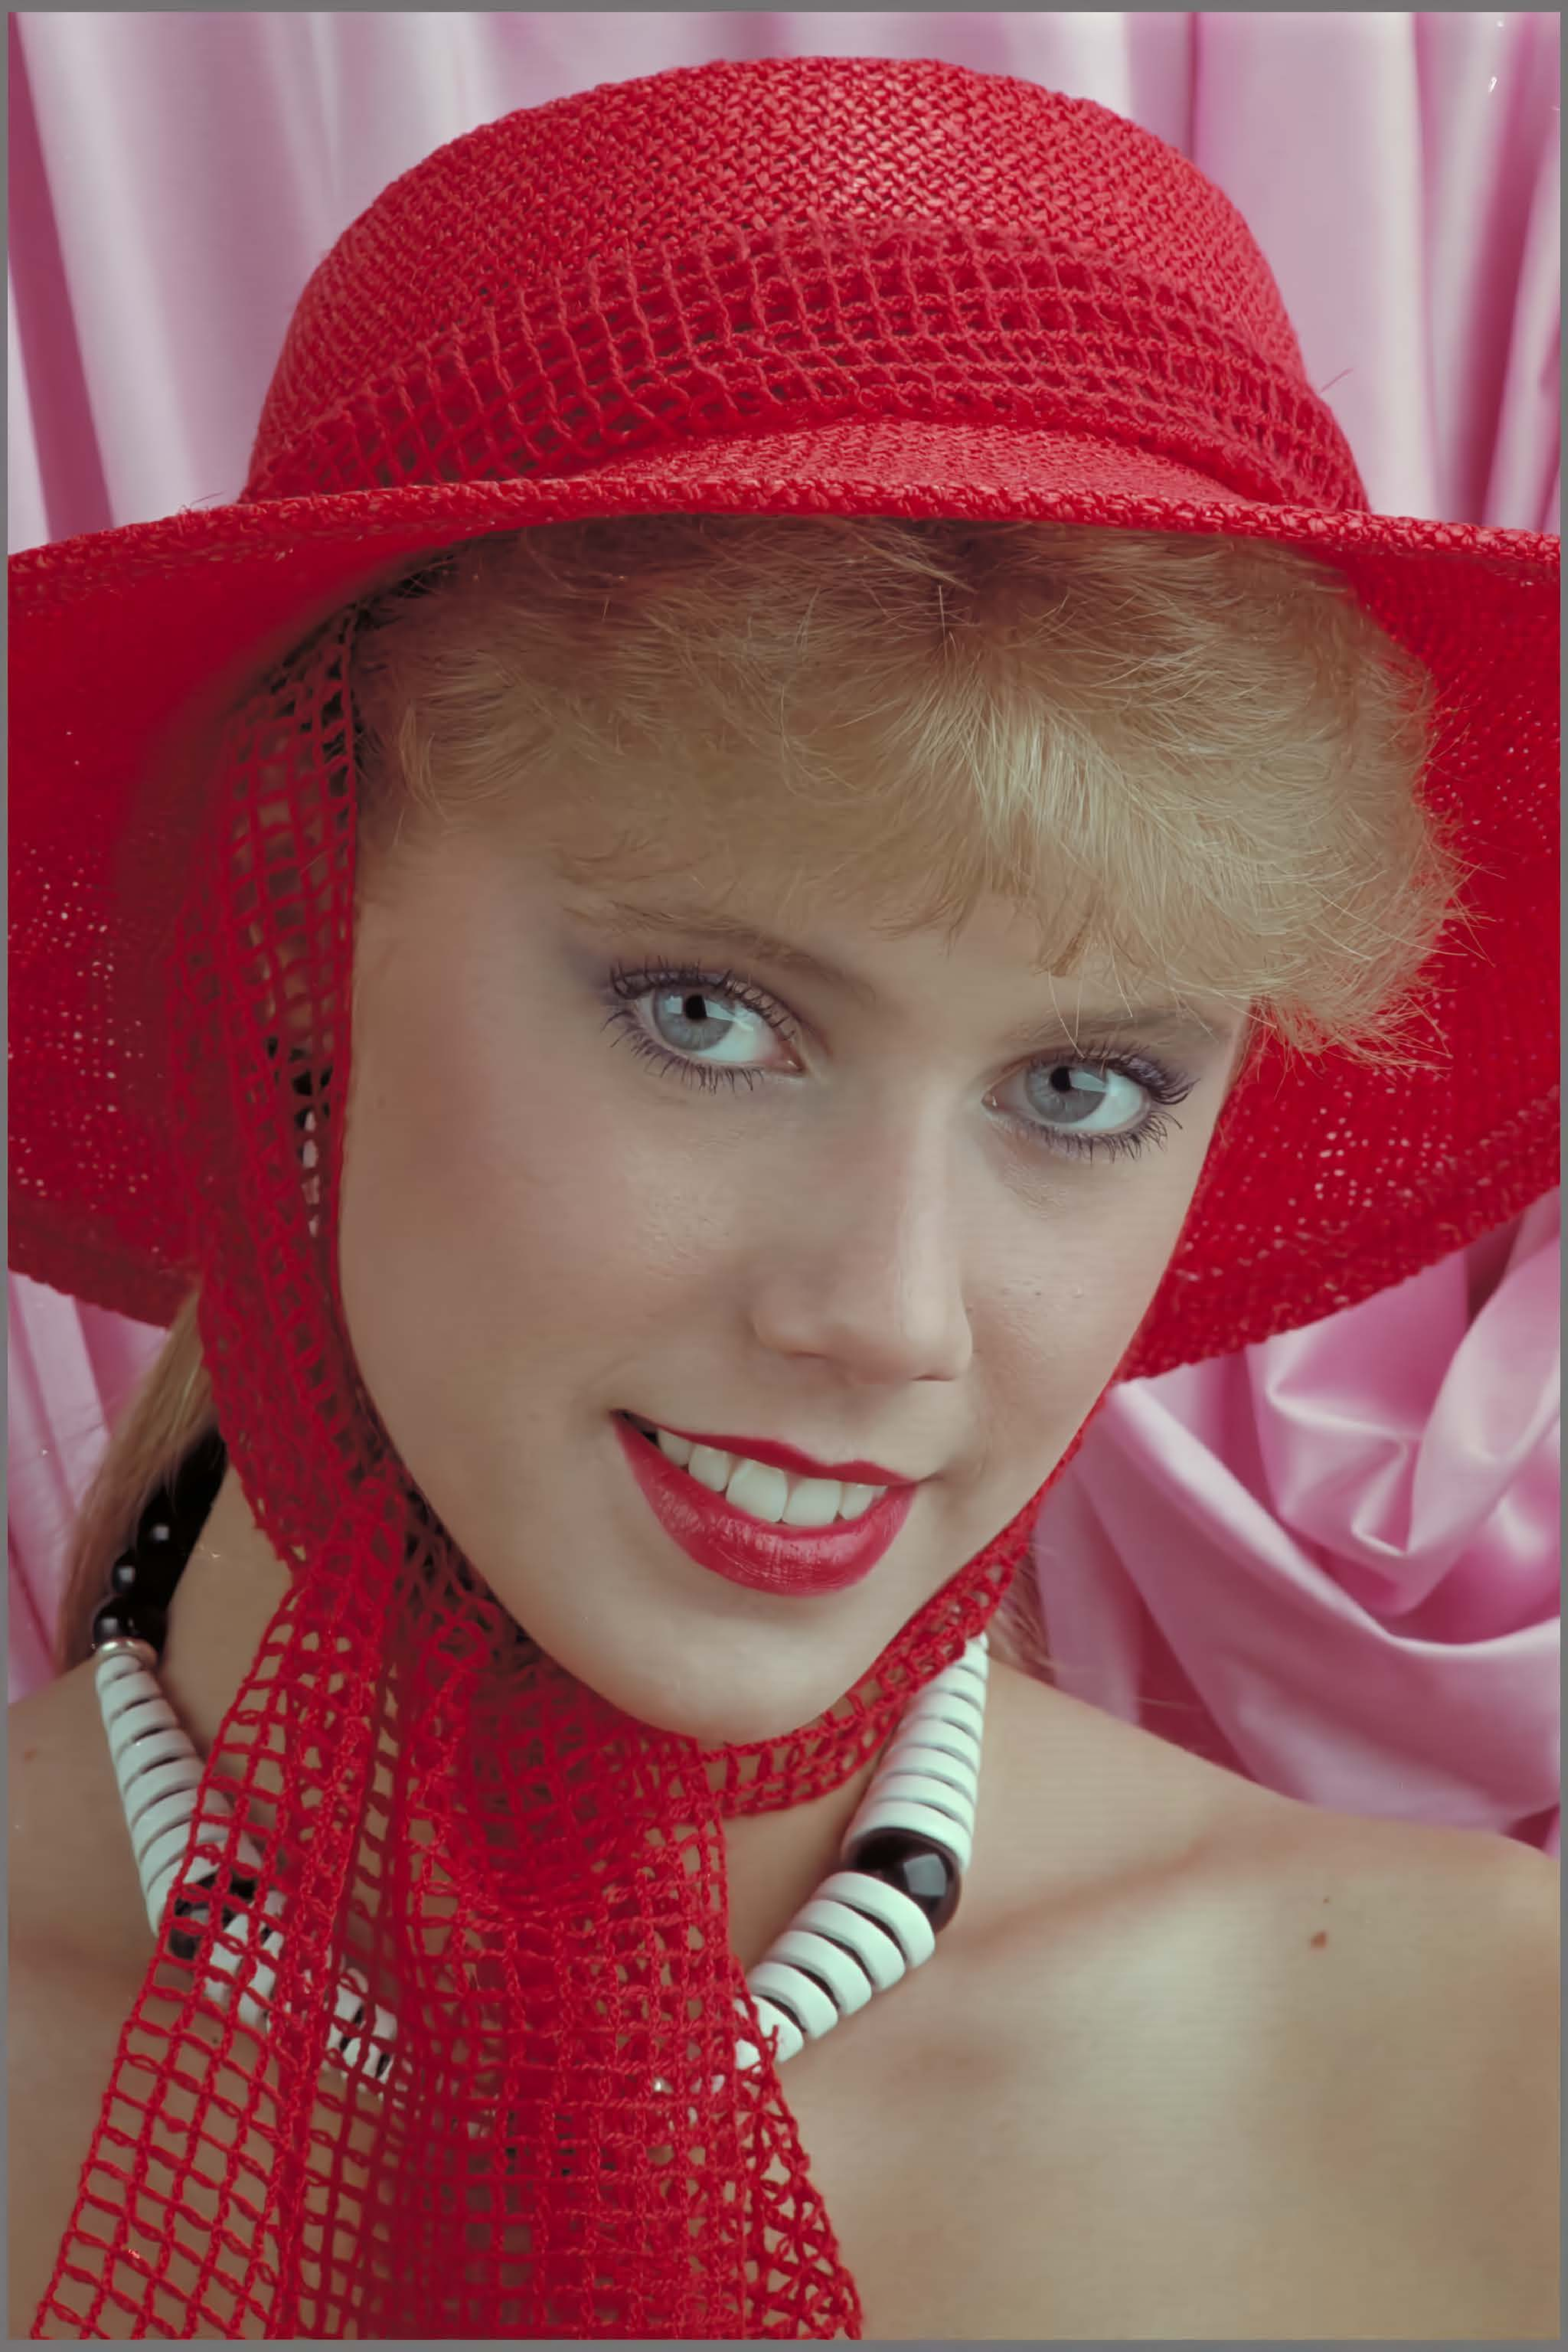
\includegraphics[width=\textwidth]{Immagini/IMAGES/cheng2020-anchor_3_IMG0004.pdf}
        \caption{Cheng2020 Attention}
        \label{fig:CompressedCheng2020Attention}
    \end{subfigure}
    \caption{Confronto PNG con Cheng2020 a 0.123 bpp}
    \label{fig:CompressionCheng2020}
\end{figure}